\documentclass{article}

\usepackage{neurips_2026}


\usepackage[utf8]{inputenc} % allow utf-8 input
\usepackage[T1]{fontenc}    % use 8-bit T1 fonts
\usepackage{hyperref}       % hyperlinks
\usepackage{url}            % simple URL typesetting
\usepackage{booktabs}       % professional-quality tables
\usepackage{amsfonts}       % blackboard math symbols
\usepackage{nicefrac}       % compact symbols for 1/2, etc.
\usepackage{microtype}      % microtypography
\usepackage{xcolor}         % colors
\usepackage{graphicx}      % for including graphics

\title{Hidden Assumptions About Tasks in Continual Learning}
%\title{What is a Task (in CL)? \\ Tasks as Discretizations of Experience}
% \title{Framework for Characterizing Task/Experience Structure in Continual/Sequential Learning}


\author{%
  Kathrin Korte \thanks{Use footnote for providing further information
    about author (webpage, alternative address)---\emph{not} for acknowledging
    funding agencies.} \\
  REAL Lab\\
  IT University of Copenhagen\\
  Copenhagen, DK \\
  \texttt{kort@itu.dk} \\
  % examples of more authors
  % \And
  % Coauthor \\
  % Affiliation \\
  % Address \\
  % \texttt{email} \\
  % \AND
  % ...
}


\begin{document}


\maketitle


\begin{abstract}

    \textbf{Abstract Draft}
    
    Continual learning research has traditionally focused on enabling agents to acquire knowledge across sequences of tasks while avoiding catastrophic forgetting. However, the field rarely examines the assumptions underlying the notion of a task itself. Existing benchmarks differ substantially in how tasks are defined, segmented, ordered, and related, yet these differences are often treated as implementation details rather than variables of scientific interest. Consequently, findings obtained on one benchmark may not readily generalize to others, despite being discussed under a common continual learning framework.
    
    We argue that many benchmark differences can be understood through hidden (or better implicit?) dimensions of experience structure, including similarity, scope, change, and exposure. Drawing on examples from continual learning and related areas such as transfer learning, curriculum learning, and concept drift, we discuss how these dimensions influence the interpretation of empirical results. We propose viewing tasks as discretizations of continuous experience rather than fundamental objects, and suggest that characterizing experience structure may provide a more principled basis for comparing benchmarks and understanding learning dynamics. Finally, we outline a research agenda toward a framework for describing task ecologies % found this formulation "task ecologies" in psychoolgy literature, not sure how well suited for this community
    and sequential experience in both artificial and biological learning systems.

\end{abstract}


% # Overview

% ### Working Motivation
%
% Continual Learning lacks a principled language for describing the structure of task
% sequences and experience streams, making it difficult to compare findings across
% benchmarks, domains, and learning paradigms. 
% Existing taxonomies primarily distinguish evaluation and learner-information scenarios, whereas we separate these from experience-stream structure and from the benchmarker’s task discretization.
%
% Current CL research often assumes:
%
% - sequence of discrete tasks exist
% - task identities are known
% - task boundaries are given
%
% while rarely discussing how these assumptions influence conclusions about:
%
% - catastrophic forgetting
% - transfer
% - replay
% - modularity
% - architecture design
% - stability-plasticity tradeoffs

% ### Goal
%
% Develop a preliminary conceptual framework for characterizing the structure of
% sequential experience and use it to analyze hidden assumptions embedded in current
% continual learning benchmarks.
%
% The goal is not yet to provide a full formal theory or definitive framework, but to:
%
% - make hidden assumptions explicit
% - identify dimensions along which benchmarks differ
% - generate hypotheses for future research
% - motivate a broader framework paper

% ### Central Claim
%
% Current continual learning benchmarks often differ along dimensions that remain
% implicit and poorly formalized.
%
% As a consequence:
%
% - findings may not generalize
% - benchmark comparisons become difficult
% - conclusions may depend on hidden properties of the task sequence rather than the
%   learning algorithm itself

% ### Some More Candidate Claims
%
% - Current CL benchmarks implicitly assume specific notions of task identity.
% - Many conclusions in CL depend on hidden properties of task sequences.
% - The field lacks a common language for describing these properties.
% - A purely task-centric view may be insufficient.
% - Tasks may be better viewed as researcher-defined discretizations of a continuous
%   experience stream.
% - Characterizing the structure of experience may be more informative than
%   characterizing tasks alone.

% ## Main Research Question
%
% Primary:
%
% "What assumptions about tasks are embedded in continual learning benchmarks, and
% what consequences do these assumptions have for the conclusions we draw?"
%
% Secondary:
%
% "What dimensions of experience structure should be explicitly considered when
% designing, comparing, and interpreting continual learning experiments?"

% ## Possible Positioning Ideas
%
% ### Beyond Task Boundaries: Hidden Assumptions About Tasks in Continual Learning
%
% Focus:
%
% - benchmark critique
% - hidden assumptions
% - task definitions
% - taxonomy
%
% ### Tasks as Discretizations of Experience: A Perspective on Continual Learning
%
% Focus:
%
% - experience-centric view
% - tasks as analytical constructs
% - preliminary framework
%
% Potentially more novel but also slightly riskier.

    
    \section{Introduction}

        Continual learning (CL) studies learning across a sequence of tasks, yet the field lacks a principled language for describing what those tasks actually are and how they relate to one another. 
        Existing taxonomies primarily distinguish evaluation and learner-information scenarios, whereas we separate these from experience-stream structure and from the benchmarker’s task discretization \cite{van2022three}.

        % Progress in continual learning has been complicated by the widespread use of the term task without a shared characterization of the assumptions that different task formulations encode.
    
        Current CL framing:
        
        Task 1 $\rightarrow$ Task 2 $\rightarrow$ Task 3

        Classical CL benchmarks typically define learning as a sequence of discrete tasks with clearly specified boundaries, such as SplitMNIST or SplitCIFAR \cite{van2022three}.     
        
        Main concerns:
        
        - catastrophic forgetting
        
        - stability-plasticity dilemma
        
        - transfer between tasks
        
        Observation:
        
        The field spends enormous effort discussing learning across tasks while rarely discussing what they even mean by task?

        Foundation-model training and deployment weaken the adequacy of the classical benchmark picture in which a learner encounters a small, externally segmented sequence of homogeneous tasks. Their data streams, adaptation stages, and usage contexts are heterogeneous, partially recurring, and often only retrospectively partitioned into tasks. (\cite{thede2024reflecting}, \cite{ostapenko2022continual})
        In \cite{zhong2026skilllearnbench} Zhong et al. introduce a benchmark for continual skill learning in LLM agents and find that benefits depend on reusable workflows.
        These works supports the claim that benchmark outcomes can be driven by representational starting conditions rather than only CL mechanisms.

        % Not sure where to fit this work but seemed relevant to me
        In \cite{riva2026taskecologiesevolutionworldtracking} Riva et al. study language models as evolving model organisms and ask when autoregressive next-token learning selects for world-tracking representations. 

        % Concrete LLM-Motivation:
            %The emergence of foundation models further challenges traditional task-centric perspectives in continual learning. In contrast to most CL Literature, modern foundation models are trained on large-scale heterogeneous data streams where such boundaries are rarely explicit. As noted by recent analyses of rehearsal-free continual learning with pretrained models \cite{thede2024reflecting}, much of the observed performance may stem from strong pretrained representations and lightweight adaptation mechanisms rather than sophisticated management of task transitions. From this perspective, task identities increasingly appear as researcher-defined abstractions imposed on an underlying continuous stream of inputs. This shift suggests that understanding the structure of experience itself may be more important than treating tasks as fundamental units of analysis.
        

        Some (predominantly recent) works show that task similarity and ordering matter in Continual learning (\cite{hiratani2024disentangling}, \cite{menghi2025impact} \cite{doan2021theoretical}, \cite{li2025optimal}). 
        Both Similarity and ordering, as well as other structural variables have been studied in specific theoretical and controlled settings, but are not yet represented in a common benchmark-description language that separates them from other CL Design Choices. 
        For example existing surveys (\cite{mendez2022reuse}) may already discuss task composition and reusable functional structure. The present work additionally claims that benchmark task definitions do not transparently specify the underlying compositional structure or the granularity of the partition allowing to draw conclusions between these choice of task design concerning these variables and a models CL Performance. 
        
        Both \cite{ostapenko2022continual} as well as \cite{thede2024reflecting} warn against simplistic claims about why CL methods work. % Also provide relevance for CL in foundation-models


        Related literature, including transfer learning, curriculum learning, online learning, and concept-drift adaptation, studies overlapping aspects of sequential experience, but the fields typically differ in units and assumptions.

        In other fields, like psychology, definitions of a task also differ. Gozli et al. \cite{Gozli2019-GOZWIA} discuss different notions of goal-directed schemata, rule-based stimulus–response organization, and depersonalized goals.
        

        % NOT SURE IF I WANT TO KEEP THIS?
        % Connection from Continual Learning (Lifelong Learning) to other fields:
        
                % \paragraph{Transfer Learning}
                
                    % - The overarching umbrella term describing the process where a model pre-trained on one task or domain is repurposed as a starting point for a different, though related, task.
                    
                    % - Example: Domain Adaptation (A subcategory of Transfer Learning) is used used when a model is trained on one dataset (the source domain) and then deployed in a new environment where the data distribution looks entirely different (the target domain), but the fundamental task % or goal (and how would we define goal? Do we need to define goal here?) 
                    % remains the same.
        
                % \paragraph{Incremental Learning} 
                
                    % - (Sometimes synonymous with Continual Learning) 
        
                    % - A Model continuously updates its knowledge sequentially, usually as new streaming data arrives, without forgetting previously learned concepts.
                
                %\paragraph{Curriculum Learning}
                
            %-  A training strategy where a model is fed data in a structured, progressive manner, starting with simple examples and moving to complex ones.     
        
        %\paragraph{Concept Drift}
                
                    % - The statistical properties of a target variable or feature shift unpredictably over time, making a static, previously accurate model degrade in performance.
                
                % All of them make either explicit or implicit % (what exactly do I mean by that?)
                %assumptions about task structure. 

        We argue that Tasks are researcher-imposed discretizations of experience streams, and many CL benchmark differences emerge from hidden properties of the underlying experience structure rather than from "tasks" themselves.   


        % Introduce a little overview over the chapters and their purposes
        Section 2 documents how current continual-learning benchmarks operationalize tasks. Section 3 abstracts from these examples to distinguish the properties of sequential learning settings that are otherwise jointly encoded in benchmark task definitions.



        Concepts:
        
        Experience stream: the temporally ordered observations, actions, labels, rewards, and contexts encountered by the learner
        
        Experience structure: regularities in that stream, such as similarity, exposure, change, and continuity
        
        Task discretization: the benchmarker’s choice to partition or label parts of the stream as tasks
        
        Learner access: which information about that partition is provided to the learner

    
    \section{How Continual Learning Currently Uses Tasks}
    
        \subsection{Benchmark Task Definitions}

        Continual-learning benchmarks use the term task for different kinds of units, including class partitions, input transformations, control goals, skill suites, and temporal distributional regimes. Table \ref{tab:task_definitions} illustrates this heterogeneity.

        \begin{table*}[t]
            \centering
            \caption{Different continual learning benchmarks implicitly adopt different notions of what constitutes a task.}
            \label{tab:task_definitions}
            \resizebox{0.75\textwidth}{!}{
            \begin{tabular}{lll}\hline
            Benchmark & What Defines a Task? & Hidden Assumption \\ \hline
            Split MNIST & Digit subset & Class partition = task \\
            Permuted MNIST & Input transformation & Differently augmented inputs imply different tasks \\
            Split CIFAR & Class partition & Semantic categories define tasks \\
            Continual World & Goal / environment configuration & Goal changes define tasks \\
            LIBERO & Robot skill suites & Skill composition defines tasks \\
            CLEAR & Experience stream & Tasks may not be explicitly defined \\
            RealCL & Continuous environment changes & Distributional regimes define tasks \\ \hline
            \end{tabular}
            }
        \end{table*}

        For example, Standard Split MNIST protocols combine class-based task partitions, blocked presentation, abrupt transitions, and often task-aware evaluation. \cite{hsu2019reevaluatingcontinuallearningscenarios}
        
        --> Add further CL Benchmarks from recent literature

        
        Main argument: Tasks are treated very differently across benchmarks.

        \subsection{Learner-access Assumptions}

        A central distinction is between how the experience stream changes and what information about that change is available to the learner. A distribution may shift abruptly or gradually irrespective of whether a task boundary is externally signaled. 
        
        Figure \ref{fig:task-based_vs_task-free} illustrates this distinction using Split MNIST. 
        
        - In the standard task-based formulation, digit subsets are presented in discrete blocks with explicit transitions. In the task-free variant, the probability of observing examples from each subset changes continuously over time. 
        
        - However, the construction still presupposes a finite set of researcher-defined underlying regimes; what is removed is primarily the explicit segmentation and task information available to the learner. 
        
        - This distinction is important because a method that succeeds without boundary signals addresses a different problem from one evaluated under the same stream with oracle task identifiers or marked transitions.

            \paragraph{Task Identity Availability}

            - known vs. unknown 
                
                % task identity and change between tasks seem to be quite intertwined here in these notions
                % how can i also make sure to properly disentangle and/or group with the notions of the boundaries paragraph
                % Is Task observability a dimension of the experience structure, or just dependent on the learner.
                % For example two experiments can have identical data, transitions, rewards and basically Identical tasks, but differ only in whether the task ID is provided.

            In CL literature this distinction is typically made between Task Incremental Learning, Domain Incremental Learning and Class Incremental Learning. These three scenarios can be distinguished based on whether, at test time, task identity is provided and, if not, whether task identity must be inferred. This means that, in theory, any sequence of tasks could be performed according to all three scenarios. \cite{van2022three}
                Figure \ref{fig:CL_scenarios} illustrates what it means for the Split MNIST toy problem to be performed according to each scenario. \cite{van_de_Ven_2025}
                
                1. Task Incremental Learning  (Easiest Scenario)
                   - task identity is strictly known and required during both training and inference.
                   - Because the model knows which task it is supposed to be solving, it typically uses multi-headed outputs or dedicated sub-networks
                
                2. Domain Incremental Learning 
                   - task identity is not available or required during inference.
                   - the set of classes remains the same, but the underlying data distribution (the "domain" or context) shifts over time (e.g., an autonomous driving system transitioning from daylight to a snowy night).
                   - model must learn to perform the same task regardless of the domain shift, usually by extracting domain-invariant features.                
                
                3. Class Incremental Learning 
                   - task identity is unknown during inference.
                   - model must predict a single, global label from all classes across all tasks it has ever encountered.
                   - relies on a single, unified output head rather than separate, task-specific ones.
                   - all tasks it has ever encountered. It relies on a single, unified output head rather than separate, task-specific ones. 
                   - Because task identity isn't provided, models typically use techniques like Knowledge Distillation or Replay Buffers (storing a small number of exemplars from past data) to prevent forgetting.
                   
        \begin{figure}[!t]
                        \centering
                        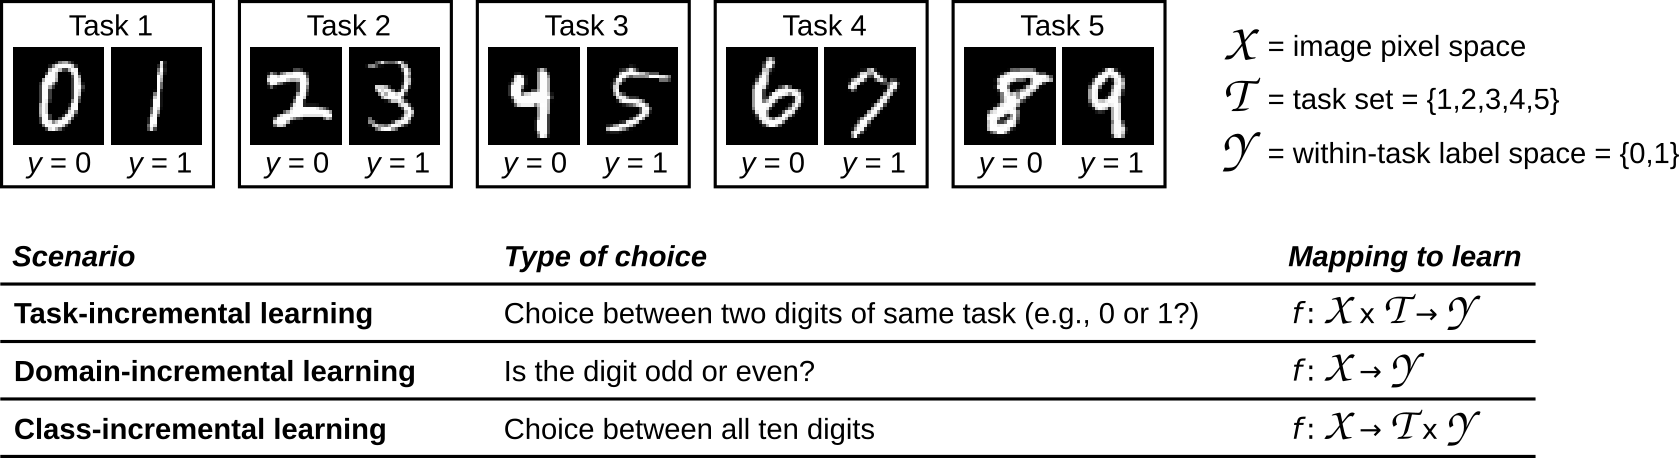
\includegraphics[width=4in]{figures/CL_scenarios.png}
                        \caption{\textbf{Split MNIST according to each of the three continual learning scenarios.} With task-incremental learning, the choice for the network is between two digits from a known task (e.g., zero or one). With domain-incremental learning, the choice is still between two options (e.g., even or odd), but the problem is more difficult as task identity is not provided. With class-incremental learning, the network must choose between all ten digits. \cite{van_de_Ven_2025}}
                        \label{fig:CL_scenarios}
                    \end{figure}



            \paragraph{Boundary Observability}
            % Task-IL / Domain-IL / Class-IL here, with qualification


             \paragraph{Task Identity}          
            
    
                - boundaries known vs unknown or gradual transitions
    
                - This concerns boundary observability: whether the learner is told that a transition occurred. This belongs under learner observability/protocol.
    
                    % Transition structure (abrupt versus gradual change) in the generating process instead belongs under Change
            
                - A common assumption in continual learning research is that there is a discrete set of tasks that are presented to the network one after the other, often with marked boundaries between tasks. \cite{van_de_Ven_2025}
    
                - This distinction is one of the paper’s clearest potential contributions. The same stream can undergo an abrupt change while the learner is not given a boundary signal; conversely, an experimenter can announce a boundary even when the distributional change is mild.

                
                - A usual categorization in COntinual Learning is between Task-based and task-free continual learning illustrated with Split MNIST. \cite{van_de_Ven_2025}
                
                BUT 
                
                - Boundary observability is not equivalent to abruptness of change. A stream can change abruptly without announcing the transition to the learner; conversely, an experimenter can mark a boundary even when the underlying change is gradual.

        % Maybe better create custom figure showing Change and Boundary observability as two independent axes
                    \begin{figure}[!t]
                        \centering
                        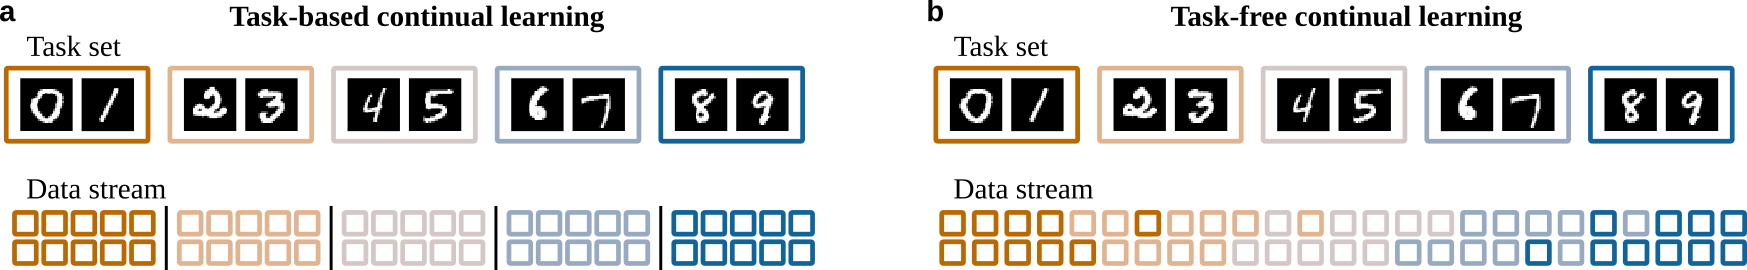
\includegraphics[width=5in]{figures/task-based_vs_task-free.png}
                            \caption{\textbf{Task-based and task-free continual learning illustrated with Split MNIST.} \textbf{(a)} In a standard task-based formulation, the dataset is partitioned into five digit-pair regimes that are presented in discrete blocks with marked transitions. \textbf{(b)} In a task-free formulation, the probabilities of observing examples from these regimes change gradually over time, without explicit boundary signals. The figure therefore contrasts both temporal transition structure and the learner's access to segmentation information; it does not imply that gradual change uniquely determines whether a task boundary exists. Adapted from \cite{van_de_Ven_2025}.}
                        \label{fig:task-based_vs_task-free}
                    \end{figure}

        The preceding examples show that benchmark names and standard CL scenarios jointly encode heterogeneous assumptions about the stream of experience, the partition used to define tasks, and the information available to the learner. 
        
        To compare findings across these settings, these assumptions must be separated rather than treated as attributes of a single object called a task. We therefore introduce a framework that allows to distinguish experience structure, task discretization, and learner access.

        Taken together, these examples show that benchmark names often bundle assumptions about task discretization, experience-stream structure, and learner access. Table~\ref{tab:benchmark_assumptions} provides an illustrative comparison across representative benchmark families.
        
            \begin{table*}[t]
                \centering
                \caption{Illustrative comparison of assumptions embedded in representative continual learning benchmarks.}
                \label{tab:benchmark_assumptions}
                \resizebox{0.99\textwidth}{!}{
                \begin{tabular}{lcccccc} \hline
                Benchmark & Task ID Known? & Boundaries Known? & Reset?& Similarity & Change & Exposure \\ \hline
                Split MNIST & Yes & Yes & Yes & Low--Medium & Abrupt & Blocked \\
                Permuted MNIST & Yes & Yes & Yes & Artificially Low & Abrupt & Blocked \\
                Split CIFAR & Yes & Yes & Yes & Medium & Abrupt & Blocked \\
                Class-IL CIFAR & No & Yes & Usually Yes & Medium & Abrupt & Blocked \\
                Continual World & Yes & Yes & Yes & Medium--High & Abrupt & Sequential \\
                CLEAR & No & No & No & Variable & Gradual & Online \\
                LIBERO & Often Partial & Variable & Mixed & High & Mixed & Sequential \\
                RealCL & No & No & No & Variable & Gradual & Online \\ \hline
                \end{tabular}
                }
            \end{table*}


            \subsection{Experience Stream Assumptions}
        
            Different benchmarks assume different notions of what makes a task, as illustrated in Table \ref{tab:task_definitions}, yet are often discussed under the same umbrella. We can categorise these Assumptions into some underlying dimensions in which they differ. % --> somehow make clear that this sohuld also concern the information that we call the experience stream, after first discussing learner-access, this is now learner independent. Probably best describe it as somhow learner-independent 
            
            % Then somehow explain first the assumptions like Task Identity, boundaries and reset and then from there \ref{tab:benchmark_assumptions} go into what we then identify as the hidden assumptions, similarity, change, exposure. Scope is already implcitly mentioned in \ref{tab:task_definitions} as "What is a Task ". So how do we get from there to merging with Scope, after introducing similarity, change & exposure first
    
    
            % Then find a way to also talk about Boundaries and Task Identity as known to the learner/model/agent
    
            Classical Notions on how to categorize Continual Learning Approaches/ Paradigms include .... 
            
            % Now decide whether to start new section or find continuation of previous assumptions to these hidden dimensions
    
            % And I think Scope should be either in the beginning of these four, or in the end, referring to the first table's "What is a Task?" but also probably as more encompassing the other dimensions???
    
            
            \paragraph{Similarity}

             % How much structure overlaps or persists between segments?
            
            The degree and type of shared structure across regions of experience
            
            - Distinguish input, output/label, latent/representational, relational/causal, and skill/policy overlap
            
            - The key literature to add here is task-similarity work, transfer/interference theory, and controlled cognitive/ANN studies (Menghi et al. and Zhang et al.) 
            
            --> manipulate structural relatedness and training regime rather than treating task order as incidental

                In \cite{johnston2023abstract} Johnston et al. show that shared task structure can induce abstraction without being explicitly imposed.
                
                In \cite{hiratani2024disentangling} Hiratani et al. Theoretical analysis showing that different forms of task similarity can have different effects on forgetting and transfer. They support the claim that overlap must be specified at the level of features, readouts, or latent structure.

                In \cite{ramasesh2020anatomy} Ramashesh et al. study catastrophic forgetting through th elens of hidden representations and task semantics therby linking forgetting patterns to semantic/representational relationships.

                In \cite{menghi2025effects} Meghi et al. compare brains and neural networks under task-similarity manipulations, focusing on representation learning and transfer/interference. % Suporting representational overlap as a relevant level of analysis.

                In \cite{hiratani2024disentangling} Hiratani analyzes how shared characteristics across tasks impact an artificial neural network's ability to retain old information and transfer knowledge.

                AS A BRIDGE TO COMPOSITIONALITY

                Then: In \cite{NEURIPS2023_6a42b45a} Liao et al. evaluate how well Continual Learning systems can recombine acquired concepts to understand new data (compositional generalization).  The paper observes that forgetting decreases when a learner has a stronger capacity for compositional generalization, as interpretable features are reused rather than overwritten.
                
                In \cite{graldi2025importance} Graldi et al. show that whether lazy or rich feature learning is preferable depends on task similarity and task non-stationarity.
                % Findings show: Rich feature learning becomes beneficial when tasks are sufficiently similar
                % The optimal amount of feature learning depends jointly on model properties and the structure of the task sequence.
                
                % For section 5: "Recent work has shown that even the optimal degree of feature learning depends jointly on model properties and task similarity, suggesting that architectural conclusions cannot be interpreted independently of the structure of the sequential learning problem. \cite{graldi2025importance}"

            \paragraph{Exposure}

            % How is experience presented, sampled and revisited?
    
            The sampling schedule conditional on the available experience
            
            - blocked/interleaved, order, spacing, frequency, recurrence, curriculum
            
            % where cognitive literature and the Menghi paper are useful
    
            - curricula matter, because identical component tasks can yield different learning dynamics under different schedules

                Bell et al. \cite{bell2022effect} demonstrates empirically that task order can substantially alter catastrophic forgetting and proposes a task-distance-based ordering method. They undermine the notion that the same task set can produce a different outcome when presented in a different schedule. 
                    % Add more literature supporting this claim

                Some works synthesize similarity and order.
                Li et al. \cite{li2025optimal} use a latent-factor teacher–student model to derive task-order principles and validate them on image benchmarks jointly formalizes similarity and ordering. Lin et al. \cite{lin2023theory} derives expected forgetting and generalization for a multi-task linear CL setting analyzing effects of overparameterization, task similarity, and order.
                
                Meghi et al. \cite{menghi2025impact} show, in both Human and neural-network experiments, that structural similarity interacts with blocked versus interleaved training regimes, the effect is asymmetric with respect to task order. 
                
                Together these works support the general proposition that forgetting is conditional on task relations and agent capacity, not a property of an algorithm alone.
                
    
            \paragraph{Change}

            % How does experience structure (the underlying distribution) evolve?
    
            The temporal geometry of the generating process: abrupt, gradual, recurrent/cyclic, or compositional change. 
            
            - Bring in concept drift and task-free CL here
            
            - treat recurrence as a bridge between change and exposure
            
            --> recurrence is an exposure property when the same distributional regime is revisited by schedule
            --> whereas cyclic drift is a change property when the generating process itself repeats
    
            % Both within and between tasks? Or mostly between?
            % Maybe in general, how do we distinguish between these dimensions within and between what is defined as a task? And do we have to, or what is the difference in effect on environment, agent and observer level?

                Figure \ref{fig:task-based_vs_task-free} illustrates why change and boundary observability should be treated separately. Gradual transitions are a property of the stream, whereas the availability of segmentation information is a property of learner access.

            Recent theoretical analyses further suggest that the optimal learning regime itself may depend on the degree of non-stationarity present in the sequential learning problem. For example, Graldi et al. \cite{graldi2025importance} show that the benefits of lazy versus rich feature learning depend jointly on task similarity and the extent of distributional change across tasks, illustrating that conclusions about learning mechanisms cannot be separated from properties of the evolving experience stream.


            \paragraph{Continuity of Interaction}


            - persistence of state, context, and interaction history across transitions
            - In interactive and embodied learning it is a very important aspect
            - whereas in supervised CL it often just reduces to a protocol convention rather than a property of the environment
            
            % Not sure, is Continuity big enough of a point to include here, or whether it is kind of related to boundaries somehow? 
            - reset vs. no reset
    
            - Reset is partly a protocol assumption and partly an environmental property, depending on the domain:
    
                - In supervised benchmarks, “reset” is mostly a metaphor for independent data partitions; there is no persistent environment state
                
                - In RL and embodied settings, reset/no-reset changes the state distribution, exploration history, reachability, and causal trajectory. There it is genuinely part of the experience ecology
    
            --> In supervised benchmarks, this denotes independence between task datasets
            --> in interactive settings, it denotes whether environmental and agent state persist across task transitions


            % REALLY NOT SURE WHERE TO PUT SCOPE HERE
            % \paragraph{Scope}
                % - Scope is a hidden design decision governing the level at which variation is grouped into a task; unlike task ID or boundary availability, it is not generally recoverable from a benchmark’s protocol alone.

                

    \section{Disentangling Sequential Learning}

        Given that benchmarks differ, what are the distinct variables needed to describe a sequential learning setting without collapsing them all into “task sequence”?

        We distinguish properties of the experience stream , the way that experience is discretized into tasks, and the information about this discretization available to the learner.
        

        % Important thatt all of these exist even if no learner is present
        
        % Potentially only these four dimensions for workshop version.
        

            \subsection{Criterion for Defining a Task}
    
            \subsection{Scope}
            
            % How much variation is grouped into a segment? (The breadth of variation grouped under a single task definition)
    
            The granularity of discretization: the breadth and heterogeneity grouped into one task
            
            % - Should naturally lead into “Tasks as Discretizations” 
        
            
            % Trying to nbe careful with difficulty:
            % Difficulty is an outcome of agent + environment + learning protocol
            % whereas scope is a property of the partition
            % They can correlate but are not interchangeable
    
            --> Scope concerns the granularity at which an observer partitions experience into units of learning, whereas difficulty concerns the resources required by a particular learner to succeed under that partition.
            
    
            Small scope: Digit 0 vs digit 1
            
            Large scope: General navigation
            
            Very large scope: Language understanding

            - task granularity
            - breadth of variation
            - heterogeneity within the partition
            - hierarchy of possible partitions
            
            % Potentially includes:
            %- sequence difficulty
            % - task difficulty
                % Task Difficulty: with clear task boundaries und reset is easier than without boundaries and reset free
            % - task granularity
            % - task hierarchy


            The work by Tang et al. \cite{tang2025importancetaskcomplexityevaluating} looks at the role of task complexity in evaluating LLM-based multi-agent systems.

            - How does task scope explain differences in CL performance?


        \subsection{Consequences for learning dynamics}

                - forgetting, transfer, interference, adaptation, abstraction, specialization, replay value, and stability–plasticity belong.

                - Agent properties should be stated here as a separate interacting factor rather than promoted to a fourth component of the benchmark framework:
                    - capacity, pretrained representatios, architecture and topology, modularity/routing, replay budget, optimization/plasticity mechanism
                    
                - Trying to formulate Learning dynamics as a function f of:
                experience structure + task discretization + learner access + agent properties
        
    \section{Tasks as Discretizations of Experience}
        
        %Potential conceptual centerpiece of the WC Paper

        % Reformulate more in line with the actual used vocabulary: "In many benchmarked learning settings, the task unit is not uniquely determined by the stream itself; it is constructed through a choice of segmentation, target, granularity, and evaluation protocol."
        
        Environment
        
        $\downarrow$
        
        Experience Stream
        
        $\downarrow$
        
        Segmentation / Discretization
        
        $\downarrow$
        
        Tasks
        
        Main idea: Tasks are not some fundamental objects but instead they may represent one particular way of partitioning continuous experience. 
        
        Discuss different Points of Views:
        --> thedifferent levels of environment/agent/observer are supposed to show why a single stream of experiences does not uniquely determine a task decomposition

        
        \subsection{Environment Level}
        
            What exists

            - latent process, state dynamics, data-generating mechanisms, objectives

        
        \subsection{Agent Level}
        
            What is experienced and represented

            1. Experienced

            - observations, actions, rewards, labels, and temporal trajectory available to an agent

            2. Represented

            - inferred contexts or representations
            - agents can for example infer different task decompositions from the same stream

            
            --> A Result of this is that task and sequence difficulty are possible consequences of the combination of overall scope with an agent
            
        
        \subsection{Observer Level}
        
            How researchers (observers) partition experience into tasks

            - segmentation, task labels, train/test partitions, evaluation
             
            % Should this section already include a lightweight dynamical systems interpretation?
            % For example:
            % - Sequence as an Experience trajectory through state space.
            % - Tasks as selected regions or segmentations of the trajectory.
        % Or maybe better keep it conceptual and void heavy mathematical formalization in workshop version.
    
    \section{Implications}

        - Implications for Benchmark Interpretation and Design

        % Conclusion
        Conclusion: 
        Continual-learning benchmarks commonly collapse several distinct layers into the label “task sequence.” They differ not only in the underlying structure of the Experience stream, but also in how that stream is externally discretized and in what information about the discretization is revealed to the learner. This conflation obscures which conditions are responsible for observed learning dynamics. Consequently, results about forgetting, transfer, or architectural suitability are conditional on a larger benchmark ecology than task labels alone capture.

        
        
        Different benchmark assumptions may lead to different conclusions regarding:
        
        - forgetting
        
        - transfer
        
        - interference
        
        - replay
        
        - modularity
        
        - architecture design
        
        - stability-plasticity tradeoffs
        
        % Do not focus only on transfer/interference
        
        The broader claim is that Learning dynamics emerge from the interaction between:
        
        - experience structure
        - agent properties

        Both \cite{johnston2024modular} show that modularity could be interpreted as an outcome of context structure rather than an architecture choice that is universally beneficial.

        Hypotheses (Examples):

        - Replay benefits may differ when past regimes recur versus never recur
        
        - Modular or routed architectures may be advantageous under low structural overlap or clear boundary cues, but unnecessary or harmful under high overlap and gradual drift

        - Apparent forgetting may reflect an evaluation protocol that requires retention of obsolete distinctions rather than a failure to preserve reusable structure
        
        - Pretraining can shift the stability–plasticity tradeoff by changing the initial representation, so comparisons between pretrained and from-scratch agents should not be interpreted solely as CL-method comparisons

        --> Different benchmarks may favor fundamentally different learning strategies


        \paragraph{Implications for Foundation Models}

        
    \section{Future Directions}
        
        Toward a framework for describing experience structure.
        
        \subsection{Formalization}
        
            Mathematical description of:
            
            - similarity
            
            - scope
            
            - change
            
            - exposure
        
        \subsection{Benchmark Taxonomy}
        
            Systematic classification of CL benchmarks.
        
        \subsection{Predictive Framework}
        
            Can these dimensions then allow us to predict:
            
            - forgetting
            
            - transfer
            
            - architecture suitability
            
            - replay requirements

        
        \subsection{Dynamical Systems View}
        
            Experience trajectories.
            
            Task segmentation.
            
            Function spaces.

            Similarity via task specific state space overlap?
            
            Connections to latent structure (complexity or scope via manifold dimensionality)
        
        \subsection{Prototype Benchmark}
        
            Long-term direction:
            
            Develop benchmark families where:
            
            - similarity
            
            - change
            
            - scope
            
            - exposure
            
            can be independently manipulated.
            
            Potentially useful for testing framework predictions.

    
    
\section{Desired Outcome of the first - Workshop Submission}
             
        Continual learning benchmarks make strong assumptions about task structure that are rarely made explicit
        
        AND
        
        A language for describing experience structure may be necessary before we can properly compare continual learning methods and draw general conclusions across benchmarks.
        
        This workshop paper should primarily serve as a problem statement, benchmark critique, and perspective piece that motivates the following conceptual framework paper.


%%%%%%%%%%%%%%%%%%%%%%%%%%%%%%%%%%%%%%%%%%%%%%%%%%%%%%%%%%%%
                        % NOTES %
%%%%%%%%%%%%%%%%%%%%%%%%%%%%%%%%%%%%%%%%%%%%%%%%%%%%%%%%%%%%

    % Similarity: a relation between regions or regimes of the experience stream. It may be measured at input, target, latent, causal, or skill level.
    % Change: how the stream’s generating process evolves over time: abrupt, gradual, compositional, cyclic.
    % Exposure: how instances of the stream are sampled and presented: order, blocking, interleaving, spacing, recurrence.
    % Continuity: whether state, interaction history, and environmental context persist across transitions. In interactive RL this is an experience-stream property; in IID supervised settings it is primarily a protocol convention.
    % Scope: a property of the discretization layer: the granularity at which heterogeneous experience is grouped into one task.
    % Task identity and boundary availability: properties of learner observability, not of the stream itself.
    % Reset: should be represented as continuity at the experience/protocol interface, rather than as a universal task property.


    % Task Observability
    % Is Task observability a dimension of the experience structure, or just dependent on the learner. 
        % For example two experiments can have identical data, transitions, rewards and basically Identical tasks, but differ only in whether the task ID is provided.
        %In CL literature this distinction is made between:
            % 1. Task Incremental Learning  (Easiest Scenario)
               % - task identity is strictly known and required during both training and inference.
               % - Because the model knows which task it is supposed to be solving, it typically uses multi-headed outputs or dedicated sub-networks
            % 2. Domain Incremental Learning 
               % - task identity is not available or required during inference.
               % - the set of classes remains the same, but the underlying data distribution (the "domain" or context) shifts over time (e.g., an autonomous driving system transitioning from daylight to a snowy night).
               % - model must learn to perform the same task regardless of the domain shift, usually by extracting domain-invariant features.                
            % 3. Class Incremental Learning 
               % - task identity is unknown during inference.
               % - model must predict a single, global label from all classes across all tasks it has ever encountered.
               % - relies on a single, unified output head rather than separate, task-specific ones.
               % - all tasks it has ever encountered. It relies on a single, unified output head rather than separate, task-specific ones. 
               % - Because task identity isn't provided, models typically use techniques like Knowledge Distillation or Replay Buffers (storing a small number of exemplars from past data) to prevent forgetting.


    \bibliographystyle{plainnat}
    \bibliography{references}

%%%%%%%%%%%%%%%%%%%%%%%%%%%%%%%%%%%%%%%%%%%%%%%%%%%%%%%%%%%%

\appendix

%\section{Technical appendices and supplementary material}
%Technical appendices with additional results, figures, graphs, and proofs may be submitted with the paper submission before the full submission deadline (see above). You can upload a ZIP file for videos or code, but do not upload a separate PDF file for the appendix. There is no page limit for the technical appendices. 

%Note: Think of the appendix as ``optional reading'' for reviewers. The paper must be able to stand alone without the appendix; for example, adding critical experiments that support the main claims to an appendix is inappropriate. 

%%%%%%%%%%%%%%%%%%%%%%%%%%%%%%%%%%%%%%%%%%%%%%%%%%%%%%%%%%%%


\end{document}